%%%%%%%%                       01 - Full Pipeline                    %%%%%%%%

\begin{frame}
  \frametitle{The Full Project Pipeline}
  \centering
  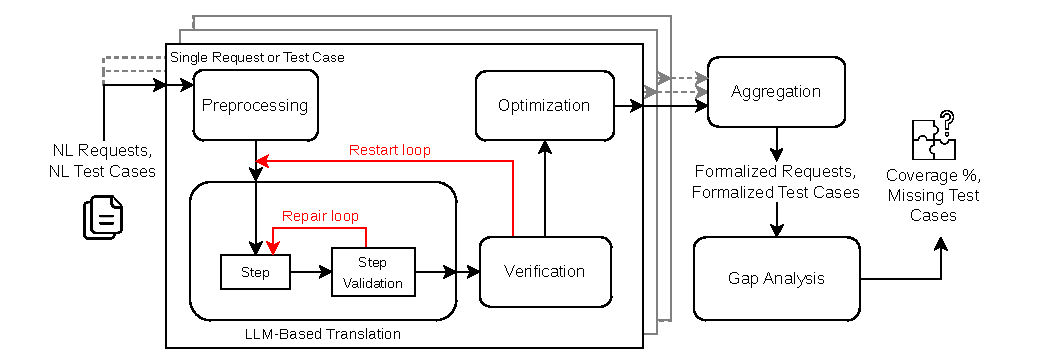
\includegraphics[width=\textwidth]{img/pipeline-overview.pdf}
  \bigskip

  \small
  Formalism $\rightarrow$
  \textbf{Translation} $\rightarrow$
  Verification $\rightarrow$ Gap Analysis
\end{frame}


%%%%%%%%                       02 - My Scope                        %%%%%%%%

\begin{frame}
  \frametitle{My Scope: NL $\rightarrow$ Formalism Translation}
  \centering
  \resizebox{\textwidth}{!}{%
  \begin{tikzpicture}[
    node distance=1.0cm and 1.2cm,
    box/.style={draw, rounded corners=4pt, minimum height=1.3cm,
      minimum width=2.4cm, align=center, font=\small\sffamily,
      fill=cyan!8, draw=cyan!40!black, line width=0.5pt},
    io/.style={draw, rounded corners=4pt, minimum height=1.1cm,
      minimum width=2.2cm, align=center, font=\small\sffamily\itshape,
      fill=gray!15, draw=gray!50, line width=0.5pt},
    validbox/.style={draw, rounded corners=4pt, minimum height=1.3cm,
      minimum width=2.4cm, align=center, font=\small\sffamily,
      fill=orange!10, draw=orange!50!black, line width=0.5pt},
    arr/.style={->, thick, >=stealth, color=gray!70!black},
    darr/.style={->, dashed, color=black!40, >=stealth},
  ]
  \node[io] (input) {NL\\Requirement};
  \node[box, right=of input] (ambiguity) {Ambiguity\\Review};
  \node[box, right=of ambiguity] (flavour) {Flavour\\Extraction};
  \node[box, right=of flavour] (entity) {Entity\\Extraction};
  \node[box, right=of entity] (formula) {Constraint\\Formalization};
  \node[validbox, right=of formula] (valid) {Structural\\Validation};
  \node[io, right=of valid] (output) {Formalized\\Requirement};

  \draw[arr] (input) -- (ambiguity);
  \draw[arr] (ambiguity) -- (flavour);
  \draw[arr] (flavour) -- (entity);
  \draw[arr] (entity) -- (formula);
  \draw[arr] (formula) -- (valid);
  \draw[arr] (valid) -- (output);

  \draw[->, thick, >=stealth, color=red!60!black]
    ([xshift=3mm]ambiguity.north) -- ++(0,0.4) -- ++(-0.8,0) -- ++(0,-0.4);
  \draw[->, thick, >=stealth, color=red!60!black]
    ([xshift=3mm]flavour.north) -- ++(0,0.4) -- ++(-0.8,0) -- ++(0,-0.4);
  \draw[->, thick, >=stealth, color=red!60!black]
    ([xshift=3mm]entity.north) -- ++(0,0.4) -- ++(-0.8,0) -- ++(0,-0.4);
  \draw[->, thick, >=stealth, color=red!60!black]
    ([xshift=3mm]formula.north) -- ++(0,0.4) -- ++(-0.8,0) -- ++(0,-0.4);

  \draw[->, thick, >=stealth, color=red!60!black]
    (valid.south) -- ++(0,-0.5) -| node[below, pos=0.25,
    font=\scriptsize\sffamily\color{red!60!black}] {retry} (formula.south);

  \draw[darr] (ambiguity.south) -- ++(0,-1.0) -|
    node[below, pos=0.15, font=\scriptsize\sffamily\color{black!40}]
    {ambiguity notes} (flavour.south);
  \draw[darr] (ambiguity.south) -- ++(0,-1.0) -| (entity.south);
  \draw[darr] (ambiguity.south) -- ++(0,-1.0) -| (formula.south west);
  \end{tikzpicture}%
  }

  \bigskip
  \small Each step: LLM call $\rightarrow$ schema validation $\rightarrow$ retry on failure
\end{frame}


%%%%%%%%                    03 - Literature Findings                  %%%%%%%%

\begin{frame}
  \frametitle{What the Literature Tells Us}
  \normalsize

  \bigskip
  \textbf{1.}\quad Structured decomposition $\rightarrow$ \textbf{+20\%} accuracy\\
  \hspace*{2em}{\small Ma et al. — REQ2LTL (aerospace, 2025),\quad Khot et al. — ICLR 2023}

  \bigskip\bigskip
  \textbf{2.}\quad Output as Python code $\rightarrow$ \textbf{3$\times$} better on frontier models\\
  \hspace*{2em}{\small Danso et al. — SecDev 2026,\quad Gao et al. — PAL, ICML 2023}

  \bigskip\bigskip
  \textbf{3.}\quad Valid structure $\neq$ correct meaning\\
  \hspace*{2em}{\small Danso et al. — temporal scoping errors dominate}
\end{frame}


%%%%%%%%                    04 - Research Questions                   %%%%%%%%

\begin{frame}
  \frametitle{Research Questions}

  \begin{enumerate}
    \item[\textbf{RQ1}] \textbf{How to decompose?}\\
    Single-call chain-of-thought vs multi-call pipeline?

    \bigskip
    \item[\textbf{RQ2}] \textbf{Output format?}\\
    JSON vs Python code — does the literature's finding hold?

    \bigskip
    \item[\textbf{RQ3}] \textbf{Model capability?}\\
    How does local vs cloud model affect the architecture choice?

    \bigskip
    \item[\textbf{RQ4}] \textbf{Which framework?}\\
    PydanticAI vs Haystack vs LangGraph vs CrewAI
  \end{enumerate}
\end{frame}


%%%%%%%%                  05 - Framework Comparison                   %%%%%%%%

\begin{frame}
  \frametitle{RQ4: Framework Comparison}
  \centering

  \small
  \renewcommand{\arraystretch}{1.4}
  \begin{tabular}{lcccc}
  \toprule
  & \textbf{PydanticAI} & \textbf{Haystack} & \textbf{LangGraph} & \textbf{CrewAI} \\
  \midrule
  Success rate & 92\% & 92\% & 75\% & 92\% \\
  Avg time & 65.0s & 65.6s & 50.5s & \textbf{25.5s} \\
  Lines of code & \textbf{$\sim$140} & $\sim$205 & $\sim$210 & $\sim$220 \\
  \bottomrule
  \end{tabular}

  \bigskip
  \small
  \textit{Model: qwen2.5:14b, 4 requirements $\times$ 3 runs each}\\
  \textit{Success = output validates against the schema (structural validity)}

  \bigskip
  \textbf{Takeaway:} Similar success rates across frameworks —
  PydanticAI simplest, CrewAI fastest.
\end{frame}


%%%%%%%%                  06 - Python vs JSON                         %%%%%%%%

\begin{frame}
  \frametitle{RQ2: Python vs JSON Output}

  \begin{columns}
  \column{0.55\textwidth}
  \centering
  \footnotesize
  \renewcommand{\arraystretch}{1.3}
  \begin{tabular}{lcc|lcc}
  \toprule
  \textbf{Req} & \textbf{J} & \textbf{Py} & \textbf{Req} & \textbf{J} & \textbf{Py} \\
  \midrule
  01 & 1/3 & 2/3 & 06 & 3/3 & 3/3 \\
  02 & 3/3 & 3/3 & 07 & 3/3 & 3/3 \\
  03 & 3/3 & 3/3 & 08 & 3/3 & 3/3 \\
  04 & 3/3 & 2/3 & 09 & 3/3 & 0/3 \\
  05 & 3/3 & 1/3 & 10 & 2/3 & 1/3 \\
  \midrule
  \multicolumn{4}{l}{\textbf{Total}} & \textbf{27/30} & \textbf{21/30} \\
  \bottomrule
  \end{tabular}

  \column{0.45\textwidth}
  \begin{itemize}
    \item JSON: \textbf{90\%}
    \item Python: \textbf{70\%}
    \item \textit{Contradicts Danso et al.}
  \end{itemize}

  \bigskip
  \small
  Literature found Python better on frontier models.
  JSON performed better on a 14B local model.

  \bigskip
  \textit{Needs further testing across model sizes.}
  \end{columns}
\end{frame}


%%%%%%%%                  07 - CoT vs Pipeline                        %%%%%%%%

\begin{frame}
  \frametitle{RQ1 + RQ3: CoT vs Pipeline}
  \centering

  \renewcommand{\arraystretch}{1.4}
  \begin{tabular}{lcccc}
  \toprule
  & \multicolumn{2}{c}{\textbf{phi4:14b (local)}} & \multicolumn{2}{c}{\textbf{Gemini 3.5 Flash}} \\
  \midrule
  \textbf{Req} & Pipeline & CoT & Pipeline & CoT \\
  \midrule
  02 & \checkmark & \checkmark & \checkmark & \checkmark \\
  03 & \checkmark & $\times$ & \checkmark & \checkmark \\
  06 & \checkmark & \checkmark & \checkmark & \checkmark \\
  09 & $\times$ & $\times$ & \checkmark & \checkmark \\
  \midrule
  \textbf{Total} & \textbf{3/4} & \textbf{2/4} & \textbf{4/4} & \textbf{4/4} \\
  \bottomrule
  \end{tabular}

  \bigskip
  \small
  Pipeline succeeded more often on the local model.\\
  Both worked on the cloud model. CoT showed better temporal precision.\\
  \textit{4 requirements, 1 run each — needs larger-scale testing.}
\end{frame}


%%%%%%%%                  08 - Ground Truth                           %%%%%%%%

\begin{frame}
  \frametitle{How Close to Ground Truth? (Req 09)}
  \scriptsize

  \begin{quote}\itshape
  ``Toggle valid\_range within 500\,ns of a write to d, if ALL:
  \begin{itemize}\setlength{\itemsep}{0pt}\setlength{\parskip}{0pt}
    \item[\textbullet] difference between last Max Peak and Min Peak of d $>$ 655
    \item[\textbullet] second write to d after Min Peak detection
    \item[\textbullet] signed value of d $>$ signed value of last d''
  \end{itemize}
  \end{quote}

  \smallskip
  \centering
  \renewcommand{\arraystretch}{1.1}
  \begin{tabular}{@{}l@{\qquad}l@{}}
  \textbf{\small Ground Truth} & \textbf{\small CoT Output} {\scriptsize(Gemini)} \\[4pt]
  \ttfamily\colorbox{green!20}{CausesWithin(} &
  \ttfamily\colorbox{green!20}{CausesWithin(} \\
  \ttfamily\quad\colorbox{green!20}{AllOf(} &
  \ttfamily\quad\colorbox{green!20}{AllOf(} \\
  \ttfamily\quad\quad\colorbox{green!20}{Happening(ev\_write\_d),} &
  \ttfamily\quad\quad\colorbox{green!20}{Happening(ev\_write\_d),} \\
  \ttfamily\quad\quad\colorbox{green!20}{Val(d, \textit{at max peak})} &
  \ttfamily\quad\quad\colorbox{yellow!30}{Val(max\_peak)} \\
  \ttfamily\quad\quad\colorbox{green!20}{\;- Val(d, \textit{at min peak}) > 655,} &
  \ttfamily\quad\quad\colorbox{yellow!30}{\;- Val(min\_peak) > 655,} \\
  \ttfamily\quad\quad\colorbox{green!20}{EvtOccCount = 2,} &
  \ttfamily\quad\quad\colorbox{green!20}{EvtOccCount = 2,} \\
  \ttfamily\quad\quad\colorbox{red!20}{Val(d) > Val(d, \textit{prev write})} &
  \ttfamily\quad\quad\colorbox{red!20}{Val(d) > ValBefore(d)} \\
  \ttfamily\quad ),  &
  \ttfamily\quad ), \\
  \ttfamily\quad\colorbox{green!20}{Val(vr) = $\neg$ValBefore(vr),} &
  \ttfamily\quad\colorbox{green!20}{Val(vr) != ValBefore(vr),} \\
  \ttfamily\quad\colorbox{green!20}{500ns} &
  \ttfamily\quad\colorbox{green!20}{500ns} \\
  \ttfamily ) & \ttfamily ) \\
  \end{tabular}

  \smallskip
  \colorbox{green!20}{\small\strut\ correct\ }\quad
  \colorbox{yellow!30}{\small\strut\ simplified\ }\quad
  \colorbox{red!20}{\small\strut\ wrong temporal ref\ }

  \smallskip
  \centering\scriptsize
  \renewcommand{\arraystretch}{1.2}
  \begin{tabular}{lccc}
  & \textbf{Gemini/pipe} & \textbf{Gemini/CoT} & \textbf{Claude/CoT} \\
  Peak diff & \cellcolor{red!20}$\times$ & \cellcolor{yellow!30}$\sim$ & \cellcolor{green!20}\checkmark \\
  Toggle & \cellcolor{red!20}$\times$ & \cellcolor{green!20}\checkmark & \cellcolor{green!20}\checkmark \\
  ``Last d'' & \cellcolor{red!20}$\times$ & \cellcolor{red!20}$\times$ & \cellcolor{red!20}$\times$ \\
  \end{tabular}
\end{frame}


%%%%%%%%                  09 - Key Findings                           %%%%%%%%

\begin{frame}
  \frametitle{Key Findings}

  \begin{enumerate}
    \item \textbf{Model capability} appears to be the strongest factor

    \bigskip
    \item \textbf{Output format} results differ from literature\\
    {\small (JSON won locally; literature reports Python wins on frontier models)}

    \bigskip
    \item \textbf{Structured decomposition} appeared to help in all tests

    \bigskip
    \item \textbf{Structural $\neq$ semantic} correctness\\
    {\small (a valid formula can still mean the wrong thing)}
  \end{enumerate}

  \bigskip
  \centering
  \small\textit{All findings are preliminary — small sample sizes, limited models.}
\end{frame}


%%%%%%%%                  10 - Open Questions                         %%%%%%%%

\begin{frame}
  \frametitle{Open Questions}

  \begin{itemize}
    \item \textbf{Pipeline granularity} — single call, multi-call, or hybrid?

    \bigskip
    \item \textbf{Semantic validation} — how to detect ``correct structure, wrong meaning''?

    \bigskip
    \item \textbf{Human-in-the-loop} — where and how much review is needed?

    \bigskip
    \item \textbf{Fine-tuning} — can corrections be accumulated to improve over time?

    \bigskip
    \item \textbf{Comprehensive evaluation} — do the observed trends hold at larger scale?
  \end{itemize}
\end{frame}


%%%%%%%%                       11 - References                        %%%%%%%%

\begin{frame}
  \frametitle{Key References}
  \scriptsize
  \begin{itemize}
    \item Ma et al., ``REQ2LTL: Bridging NL and Formal Specification
    via Hierarchical Semantics Decomposition Using LLMs,'' 2025
    \item Danso et al., ``Syntax Is Easy, Semantics Is Hard:
    Evaluating LLMs for LTL Translation,'' ACM SecDev, 2026
    \item Khot et al., ``Decomposed Prompting: A Modular Approach
    for Solving Complex Tasks,'' ICLR, 2023
    \item Gao et al., ``PAL: Program-Aided Language Models,''
    ICML, 2023
    \item Cosler et al., ``nl2spec: Interactively Translating
    Unstructured NL to Temporal Logics with LLMs,'' CAV, 2023
    \item Xu et al., ``Learning from Failures: Translation of NL
    Requirements into LTL with LLMs,'' IEEE QRS, 2024
    \item Nouri et al., ``Engineering Safety Requirements for
    Autonomous Driving with LLMs,'' IEEE RE, 2024
    \item Beg et al., ``A Systematic Literature Review on
    Formalising NL Requirements Using LLMs,'' 2025
    \item Ahmed \& Wei, ``DDL2PropBank Agent: Benchmarking
    Multi-Agent Frameworks,'' 2026
  \end{itemize}
\end{frame}


%%%%%%%%                       12 - Thanks                            %%%%%%%%

\begin{frame}
  \frametitle{Thank You for Your Attention!}
  \centering

  \resizebox{\textwidth}{!}{%
  \begin{tikzpicture}[
    node distance=1.0cm and 1.2cm,
    box/.style={draw, rounded corners=4pt, minimum height=1.3cm,
      minimum width=2.4cm, align=center, font=\small\sffamily,
      fill=cyan!8, draw=cyan!40!black, line width=0.5pt},
    io/.style={draw, rounded corners=4pt, minimum height=1.1cm,
      minimum width=2.2cm, align=center, font=\small\sffamily\itshape,
      fill=gray!15, draw=gray!50, line width=0.5pt},
    validbox/.style={draw, rounded corners=4pt, minimum height=1.3cm,
      minimum width=2.4cm, align=center, font=\small\sffamily,
      fill=orange!10, draw=orange!50!black, line width=0.5pt},
    arr/.style={->, thick, >=stealth, color=gray!70!black},
    darr/.style={->, dashed, color=black!40, >=stealth},
  ]
  \node[io] (input) {NL\\Requirement};
  \node[box, right=of input] (ambiguity) {Ambiguity\\Review};
  \node[box, right=of ambiguity] (flavour) {Flavour\\Extraction};
  \node[box, right=of flavour] (entity) {Entity\\Extraction};
  \node[box, right=of entity] (formula) {Constraint\\Formalization};
  \node[validbox, right=of formula] (valid) {Structural\\Validation};
  \node[io, right=of valid] (output) {Formalized\\Requirement};

  \draw[arr] (input) -- (ambiguity);
  \draw[arr] (ambiguity) -- (flavour);
  \draw[arr] (flavour) -- (entity);
  \draw[arr] (entity) -- (formula);
  \draw[arr] (formula) -- (valid);
  \draw[arr] (valid) -- (output);

  \draw[->, thick, >=stealth, color=red!60!black]
    ([xshift=3mm]ambiguity.north) -- ++(0,0.4) -- ++(-0.8,0) -- ++(0,-0.4);
  \draw[->, thick, >=stealth, color=red!60!black]
    ([xshift=3mm]flavour.north) -- ++(0,0.4) -- ++(-0.8,0) -- ++(0,-0.4);
  \draw[->, thick, >=stealth, color=red!60!black]
    ([xshift=3mm]entity.north) -- ++(0,0.4) -- ++(-0.8,0) -- ++(0,-0.4);
  \draw[->, thick, >=stealth, color=red!60!black]
    ([xshift=3mm]formula.north) -- ++(0,0.4) -- ++(-0.8,0) -- ++(0,-0.4);

  \draw[->, thick, >=stealth, color=red!60!black]
    (valid.south) -- ++(0,-0.5) -| node[below, pos=0.25,
    font=\scriptsize\sffamily\color{red!60!black}] {retry} (formula.south);

  \draw[darr] (ambiguity.south) -- ++(0,-1.0) -|
    node[below, pos=0.15, font=\scriptsize\sffamily\color{black!40}]
    {ambiguity notes} (flavour.south);
  \draw[darr] (ambiguity.south) -- ++(0,-1.0) -| (entity.south);
  \draw[darr] (ambiguity.south) -- ++(0,-1.0) -| (formula.south west);
  \end{tikzpicture}%
  }

\end{frame}
